%&latex
%
\documentclass[../template.tex]{subfiles}
\usepackage{amsbsy}

\begin{document}

\section{Course information} %computational physics
\lesson{1}{3/10/2019}
%Password moodle: NPhyS-2019.\\
%App Socrative Student. Course: Lenzinp.
The goal of this course is to introduce a series of problems in modern physics (in particular of statistical mechanics), describing their origin and their solution, along with some useful mathematical tools. At the end of the lectures, one student should be able to formulate problems and solve them. Exercises will be published online, and the final exam will consist of a theoretical question and a problem to solve (similar to the ones seen during the course). It will be needed to bring an \textit{exercise book} with all the written solutions of the course's exercises.\\
%Goals and modality need to be known for the exam


\section{Introduction}
In classical mechanics, if we know all forces $\vec{F}$ that act on a certain particle, along with its initial condition (e.g. position $\vec{x}(t=0)$ and velocity $\vec{v}(t=0)$), we can compute its trajectory $\vec{x}(t)\> \forall t$ by integrating the equations of motion.\\
This is indeed true even for ensembles of particles - but it becomes very impractical for macroscopical objects. For example, a drop of water contains something in the order of $10^{23}$ molecules, and so to completely describe its motion it is needed to integrate six times that many equations ($3$ for position, $3$ for velocity for each single particle). Even if we had the computational capacity to do so, it would not be possible to know the necessary initial conditions with the required precision.\\

On the other hand, it is not very interesting to solve this kind of problem, because one could not possibly understand the intricacy of this motion, and so the task doesn't give much insight in the relevant physics. In fact, often we are most interested in the \textit{macroscopical} properties of the object. That is the aim of \textit{statistical mechanics}.

\section{The diffusion problem}
We start by considering a famous problem in statistical mechanics, the \textit{diffusion problem}, which consists in describing what happens to a droplet of fluid in a bath of a different substance (e.g. ink in water).\\

There are two main results about diffusion:
\begin{itemize}
\item Fick's Law ($\sim 1895$)
\item Einstein's paper on brownian motion ($1905$). 
\end{itemize}

\subsection{Brownian motion}
The explanation of brownian motion proposed by Einstein in $1905$ was the first demonstration of the discrete nature of matter, i.e. the fact that substances are made of smaller discrete particles: molecules.\\
Einstein observed that a fine powder, not containing any \textit{living organisms}, moved erratically if suspended in still water.\\

If we assume that water is composed of particles, the single grains of powder behave like large objects hit by smaller particles. The number of hits on each side is almost the same, so the total force which acts on the large object is almost $0$. However, if the grains are sufficiently small, the slight unbalance in the number of collisions can produce a significant acceleration, leading to a kind of \textit{random motion}.\\

For example, let's consider a spherical grain submerged in the liquid. Let's call $U$ the upper emisphere, and $L$ the lower one. Denote with $\bar{N}_c$ the average number of collisions per second per surface unit. Then the number of hits on $U$ is \textit{almost} the same to that of $L$, up to a certain (binomial) error:
\begin{align*}
\bar{N}_c \cdot U = \bar{N}_c \cdot L \pm \sqrt{\bar{N}_c}
\end{align*}
Thus, the relative error is given by:
\begin{align*}
    \frac{\sqrt{\bar{N_c}}}{\bar{N}_c} = \frac{1}{\sqrt{\bar{N}_c}}  
\end{align*}
Note that if the grains are small, $\bar{N}_c$ will be small too, and so the relative error will be high.

\subsection{Time evolution and the continuity equation}
Let's try to give a quantitative description of this kind of motion. We start by specifying the \textit{initial conditions} as a \textit{starting distribution}, i.e. a function $\rho\colon \mathbb{R}^3 \times \mathbb{R} \to R$ such that $\rho(\vec{r},t)$ is the probability to find a particle in position $\vec{r}$ at the instant $t$. \marginpar{Starting distribution}
\begin{enumerate}
\item For a discrete, point particle we have $\rho(\vec{r},0)=\delta^3(\vec{r}-\vec{r}_0)$, i.e. the particle is at the starting position with certainty.
\item For some quantity of matter (for example a droplet of ink), we have some uniform initial density, such as:
\begin{align*}
\rho(\vec{r},0) = \rho_0(\vec{r}) = \begin{cases}
\bar{\rho}_0 & |\vec{r}\,|<R\\
0 & \text{otherwise}
\end{cases}
\end{align*}
\end{enumerate}
Note that $\rho(\vec{r},t)$ is a probability density, and not a usual density of matter. The difference is merely of normalization. If $N$ is the total number of particles in ink, then $N\rho(\vec{r},t)$ is the density of ink particles at \textit{the specific} position $\vec{r}$ and time $t$, which will be denoted with $\rho_n(\vec{r},t)$:
\begin{align*}
1 &= \int_V \dd[3]{r} \rho(\vec{r},t)\\
N &= \int_V \dd[3]{r} \underbrace{N\rho(\vec{r},t)}_{\text{density at $\vec{r}$}}
\end{align*}
The meaning of a point-wise density can be understood as a limit:\marginpar{Point-wise density}
\begin{align*}
N \rho(\vec{r},t) = \text{density at $\vec{r}$, time $t$} = \lim_{\Delta V \downarrow 0} \frac{\Delta N}{\Delta V}
\end{align*}
Consider a patch of liquid of volume $\Delta V$, that contains a number $\Delta N$ of ink particles. By letting it shrink \q{enough}, $\Delta N/\Delta V$ reaches a constant value - that is the density in a macroscopically small patch of liquid. Of course, $\Delta V$ cannot reach $0$, because in that case $\Delta N = 0$. So, the limit is to be interpreted in a macroscopical sense ($\Delta V$ is macroscopically vanishing, $\Delta V \downarrow 0$) and not in a mathematical sense ($\Delta V \to 0$).

\begin{minipage}[t]{0.45\textwidth}
\begin{figure}[H]
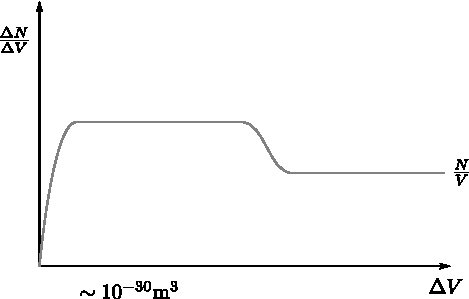
\includegraphics[width=\textwidth]{Plots/patch_centered_ink.pdf}
\caption{Density (ratio $\Delta N/\Delta V$) as function of patch size $\Delta V$ for a region centered around the ink distribution $\rho_0$ ($|\vec{r}|<R$ at $t=0$). If $\Delta V$ is sufficiently large, the patch comprises also some space without ink, and so the density is lower.}
\end{figure}
\end{minipage}\hfill%
\begin{minipage}[t]{0.45\textwidth}
\begin{figure}[H]
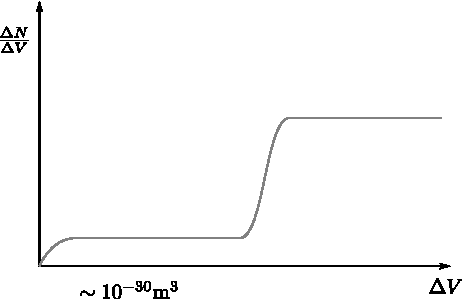
\includegraphics[width=\textwidth]{Plots/patch_centered_not_ink.pdf}
\caption{Density for a patch centered on a point $|\vec{r}|>R$. Here the density is higher for high $\Delta V$, as in these cases the patch comprises also the ink's initial distribution ($\rho_0$).}
\end{figure}
\end{minipage}

We now want to compute $\rho(\vec{r},t)$ for $t>0$, given $\rho(\vec{r},0)$.\\
We start by considering the \textit{continuity equation}.\marginpar{Continuity equation} The idea is that particles do not move by \q{jumping} between far positions, but travel in a \textit{continuous way}.\\

Consider a box of volume $V$, that contains a fixed number $N$ of particles, with density:
\begin{align*}
N\rho(\vec{r},t) \equiv \rho_n(\vec{r},t)
\end{align*}
Let $A$ be a patch of $V$, with boundary $\partial A$. The number of particles inside $A$ at time $t$ is given by:
\begin{align}
\int_A \dd[3]{r} \rho_n(\vec{r},t) &= N_A(t)
\label{eqn:N-A}
\intertext{And at a later time $t+\Delta t$:}
\int_A \dd[3]{r}\rho_n(\vec{r},t+\Delta t) &= N_A(t+\Delta t)
\label{eqn:N-A-deltat}
\end{align}
Let's introduce a new quantity, the \textit{current} $\vec{j}(\vec{r},t)$ at position $\vec{r}$ and time $t$. 
Consider a small area $\dd{S}$ centered on $\vec{r}$, with $\hat{n}(\vec{r}) \perp \dd{S}$. The number of particles flowing through $\dd{S}$ during an interval $\Delta t$ is defined as:
\begin{align*}
\Delta t \vec{j}(\vec{r},t) \cdot \hat{n}(\vec{r}) \dd{S}
\end{align*}
and this can be used to compute $\vec{j}$.\\
For example, for a uniform flow of particles with density $\rho_n$ and velocity $\vec{v}$, the \textit{current} is $\vec{j} = \rho_n \vec{v}$.\\

Returning to the problem, we note that the \textit{change} of $N_A$ over time is explained by the \textbf{flux} of particles through the closed boundary $\partial A$, i.e. the surface integral of the current $\vec{j}$:
\begin{align}
N_A(t+\Delta t) - N_A(t) = - \int_{\partial A} \dd{S} \hat{n}\cdot \vec{j}(\vec{r},t)\Delta t
\label{eqn:change-N}
\end{align}
Here we define, by convention, the sign of $\vec{j}(\vec{r},t)$ to be positive if the current is \textit{outward}, that is from $A$ to $V\setminus A$. So, a positive current means that particles are \textit{leaving} $A$, and this explains the $-$ in (\ref{eqn:change-N}).\\

Substituting (\ref{eqn:N-A}) and (\ref{eqn:N-A-deltat}) in (\ref{eqn:change-N}) we arrive at:
\begin{align*}
\int_A \dd[3]{r} \frac{1}{\Delta t} \left[\rho_n(\vec{r},t+\Delta t)- \rho_n(\vec{r},t) \right] = -\int_{\partial A} \dd{S}(\vec{r}) \vec{j}(\vec{r},t)\cdot \hat{n}(\vec{r}) \cancel{\Delta t}
\end{align*}
Taking the limit $\Delta t\to 0$:
\begin{align*}
\int_A \dd[3]{r} \frac{\partial}{\partial t}\rho_n(\vec{r},t) = -\int_{\partial A} \dd{S} \hat{n} \cdot \vec{j}(\vec{r},t) \underset{(a)}{=} - \int_A \dd[3]{r} \vec{\nabla} \cdot \vec{j}(\vec{r},t)
\end{align*}
where in (a) we applied the Gauss divergence theorem.\\
Rearranging:
\begin{align*}
\int_A d^3r [\dot{\rho}_n(\vec{r},t) + \vec{\nabla}\cdot \vec{j}(\vec{r},t)] = 0
\end{align*}
This is the \textbf{continuity equation} in integral form. Note that it holds for any choice of volume $A \subseteq \mathbb{R}^3$. So, knowing that $\vec{j}$ and $\dot{\rho}$ are continuous functions, by the fundamental theorem of calculus we know that the same relation must hold everywhere \textit{for the integrand}, meaning that:   
\begin{align}
\dot{\rho}_n (\vec{r},t) + \vec{\nabla} \cdot \vec{j}(\vec{r},t) = 0 \qquad \forall \vec{r}, \forall t
\label{eqn:continuity}
\end{align} 
That is the \textbf{continuity equation} in differential form.\\

\subsection{Fick's Law}
If there are no other fields (EM, gravity, etc.), but we still observe a non-zero $\vec{j}$, where could it possibly be from?\\
The only other relevant physical vector in this situation, i.e. not depending on an arbitrary choice of reference frame, is the \q{spatial} rate of change of density, i.e. its gradient $\vec{\nabla}\rho_n$. In fact, it is observed that particles tend to move \textit{opposite} to that gradient - from regions where there are more particles to regions where there are less. This can be summarized by \textbf{Fick's Law}:
\begin{align}
\vec{j}(\vec{r},t) = -D\vec{\nabla} \rho_n(\vec{r},t)
\label{eqn:fickslaw}
\end{align}
Of course, there could be some other terms in this expression:
\begin{align*}
\vec{j}(\vec{r},t) = -D\vec{\nabla} \rho_n(\vec{r},t) + C\vec{\nabla}(\vec{\nabla}\rho_n) + \dots
\end{align*}
However, by dimensional analysis, $\partial_x^k \rho_n \sim \rho_n/L^k$, where $L$ is the macroscopic dimension of the container. So, the higher order terms can be considered negligible.

\subsection{The Diffusion Equation}
Substituting (\ref{eqn:fickslaw}) in (\ref{eqn:continuity}) we arrive finally at the \textbf{diffusion equation} :
\begin{align}
\dot{\rho}_n(\vec{r},t) = \vec{\nabla}(D \cdot \vec{\nabla}\rho_n(\vec{r},t))
\label{eqn:evolution}
\end{align}
Knowing the initial density $\rho_n(\vec{r},0)$ and some macroscopical details for the fluids (all contained in the \textit{diffusion parameter} $D$), we can now compute the density after a small interval $\Delta t$. For example, we can start by expanding $\rho_n(\vec{r},\Delta t)$ around $\Delta t = 0$:
\begin{align*}
\rho_n(\vec{r},\Delta t) = \rho_n(\vec{r},0) + \Delta t\dot{\rho}_n(\vec{r},0) + O(\Delta t^2)
\end{align*}
Ignoring the higher order terms, we can use (\ref{eqn:evolution}) and compute $\rho_n(\vec{r},\Delta t)$.\\

This may be more or less doable depending on the form of $D$, that can depend on both $\vec{r}$ and $t$. The $\vec{r}$-dependence is characteristic of problems that are not translational invariant (e.g. a crystal). In fact, if $D$ \textbf{does not} depend on $\vec{r}$, the diffusion equation becomes:
\begin{align}
    \dot{\rho}_n(\vec{r},t) = D \nabla^2 \rho_n(\vec{r},t)
    \label{eqn:evolution-simple}
\end{align}
Because the only spatial derivatives are of second order, then if $\rho(\vec{r},t)$ is a solution, also $\rho(\vec{r}+ \vec{R},t)$ is a solution, for any choice of $\vec{R}$.\\

Note that (\ref{eqn:evolution-simple}) is quite similar to the Schr\"odinger equation for a free particle:
\begin{align*}
\hlc{ForestGreen}{-i} \partial_t \psi = +\hlc{Yellow}{\frac{\hbar}{2m}\nabla^2} \psi
\end{align*}
The yellow term is analogous to $D$, and the only difference is given by the green term. This can be resolved by a substitution $\tau = it$ (passing to \q{imaginary time}).

\begin{example}[Particle diffusing in $d=1$]
Consider the simplest case of a single particle moving in one dimension, with $D$ constant. Let $\rho(x,0) = \delta (x)$.\\
The diffusion equation in $d=1$ is: 
\begin{align}
\dot{\rho}(x,t) = D\rho''(x,t)
\label{eqn:diffusion-1d}
\end{align}
The macroscopic quantities of interest are the expected position and velocity, defined as:
\begin{align*}
\langle x\rangle_t = \int_{-\infty}^{+\infty} \rho(x,t) x\dd{x} \qquad \frac{d\langle x\rangle_t}{dt} = \int_{-\infty}^{+\infty} \dot{\rho}(x,t)x\dd{x}
\end{align*}
From the normalization condition:
\begin{align*}
\int_{-\infty}^{+\infty} \rho(x,t) dx = 1
\end{align*}
we note that $\rho(\pm \infty,t) = 0$, and also $\rho'(x,t) \to 0$ for $|x|\to \infty$ (otherwise, the density would diverge).\\
These limits allow us to compute the velocity by repeated integration by parts:
\begin{align*}
    \dv{\langle x \rangle_t}{t} &= \dv{t} \int_{-\infty}^{+\infty} \rho(x,t) x \dd{x} = 
    \int_{-\infty}^{+\infty} \dot{\rho}(x,t) x \dd{x} \underset{(\ref{eqn:diffusion-1d})}{=}  D\int_{-\infty}^{+\infty} \rho''(x,t)x \dd{x} = \\
    &= \underbrace{x \rho'(x,t)\Big|_{x=-\infty}^{x=+\infty}}_{=0}  \underbrace{-\left(\dv{x}{x}\right)\rho(x,t)\Big|_{x=-\infty}^{x=+\infty}}_{=0}  +
    D \int_{-\infty}^{+\infty} \rho(x,t)\underbrace{\left(\dv[2]{x}{x}\right)}_{=0}\dd{x} = 0
\end{align*}
A similar calculation can be done for the expected value of the time derivative of a generic function $f(x)$:
\begin{align}
    \dv{t}\langle f(x) \rangle = D \int_{-\infty}^{\infty} \rho(x,t) \left(\dv[2]{f(x)}{x}\right) \dd{x}
    \label{eqn:expected-f}
\end{align} 
As the velocity is $0$, the position is constant, so that:
\begin{align*}
    \langle x \rangle_t = \langle x \rangle_{t=0} = \int_{-\infty}^{+\infty} \dd{x} x \rho(x,0) = 0
\end{align*}

However, if we consider $f(x) = x^2$, thanks to (\ref{eqn:expected-f}) we arrive at:
\begin{align*}
    \dv{t} \langle x^2 \rangle_t = \int_{-\infty}^{+\infty}\dot{\rho}(x,t) x^2 \dd{x} = D \int_{-\infty}^{+\infty} 2 \rho(x,t) \dd{x}
\end{align*}
As $\rho(x,0) = \delta(x)$, we have:
\begin{align*}
    \dv{t}\langle x^2 \rangle_0 = D \int_{-\infty}^{+\infty} 2\delta(x) \dd{x} = 2D
\end{align*}  
And integrating with respect to $t$:
\begin{align*}
    \langle x^2 \rangle_t = 2D t + \langle x^2 \rangle_0 = 2Dt
\end{align*} 
\end{example}
\end{document}


